\section{Robustness analysis}

\todo[inline]{This section is not complete@@@}
Even though the system is stable with the model that has been given, the assumptions that were made may be somewhat incorrect. As a result, the constructed controller should preferably also have at least some robustness against modelling errors. This analysis will only focus on errors in input gain and on time-delays. All models described in this section will be of continuous LTI systems. 


\subsection{Combined estimator and physical system}

The physical plant, and the one used by the MPC are not entirely the same. As a result, some extra steps have to be taken when representing both the physical system and the estimated one in the same state-space. This analysis will only go over input-delays and not output-delays. 


\noindent
Let $A$,$B_p$,$C$ and $D$ represent the physical system and the matrix $B$ input matrix of the estimated system. Finally, let $K_{lqe}$ represent the feedback mmatrix used by the linear quadratic estimator.  Then the open-loop system between the real state and the estimated state can be written as:

\begin{align}
    \begin{bmatrix}
        x\\
        \hat{x}
    \end{bmatrix}
    = 
    \begin{bmatrix}
        A & 0 \\
        K_{lqe} C & A - K_{lqe} C
    \end{bmatrix}
    \begin{bmatrix}
        x\\
        \hat{x}
    \end{bmatrix}
    + 
    \begin{bmatrix}
        B_p\\
        B
    \end{bmatrix}
    u
\end{align}

The controlled system is not necessarily the same as the estimated system. A low-pass filter has to be used by the controller or estimator to make remove all feed-through terms from LTI-system. This low-pass filter is represented by the matrices $A_F$ , $B_F$ and $C_F$. Additionally, the controlled states are not necessarily the same as the measured outputs, so a different pair of matrices $C_c$ $D_c$ are used to axtract them form the estimate. Said measurements are used for making the integrator states of the plant. Finally, a padé-approximation is needed for the delay between the input-filter and the rest of the process. The delay will be estimated by $A_D$, $B_D$, $C_D$ and $D_D$. 

The full system is divided into several smaller sub-systems. 
\begin{align}
    x_{full}
    \begin{cases}
        x_{\text{physical}}\\
        x_{\text{estimated}} \\
        x_{\text{input filter}}\\
        x_{\text{integrated outputs}}\\
        x_{\text{padé approxomation}}\\
    \end{cases}
\end{align}

\begin{align}
    A_{full} 
    = 
    \begin{bmatrix}
        A        & 0            & B_p D_D C_{F} & 0   & B_p C_D          \\
        K_{lqe}C & A - K_{lqe}C & B C_F         & 0   & 0           \\
        0        & 0            & 0             & A_F & 0         \\
        C_c      & 0            & D D_D C_F     & 0   & D C_D   \\
        0        & 0            & B_D C_F       & 0   & A_D   \\
    \end{bmatrix}
\end{align}

\begin{align}
    B_{full}   =
    \begin{bmatrix}
        0 \\
        0 \\
        B_F \\
        0 \\
        0
    \end{bmatrix}
\end{align}

Instead of using normal states as outputs, it is also possible to translate them directly into the corresponding optimal set of inputs. The matrix $K_{lqr}$ uses the estimated states, as well as the filtered states and the integrated states. 

\begin{align}
    C_{full} = 
    \begin{bmatrix}
        0 & K_{lqr} & 0
    \end{bmatrix}
\end{align}

Because of the low-pass filter, $D_{full}$ is always 0. The stability of the feedback loop can be analysed by adding a padé approximation of a delay in the feedback between the optimal next input given out by $C_{full}$ and the input used on $B_{full}$. 
\noindent

\subsection{The root locus plots}
With a fully functioning state-space system of both the physical system and the estimated one, it becomes possible to say something about how the poles evolve, depending on delay and static gain error. To test the static gain error, it is simply sufficient to multiply $B_p$ 
by some constant. The robustness to delay can be tested by adding a padé- approximation in the feedback-loop, of some pre-determined order, and then setting the desired delay. In this analysis, order 9 was chosen, although there may be reasons for choosing other padé-approximations as well. 

In this section, the LQR-controller with integral cost on $F_{aI} - F_{aII}$ will be covered, since it was one of the best-performing architectures. 

\begin{figure}
    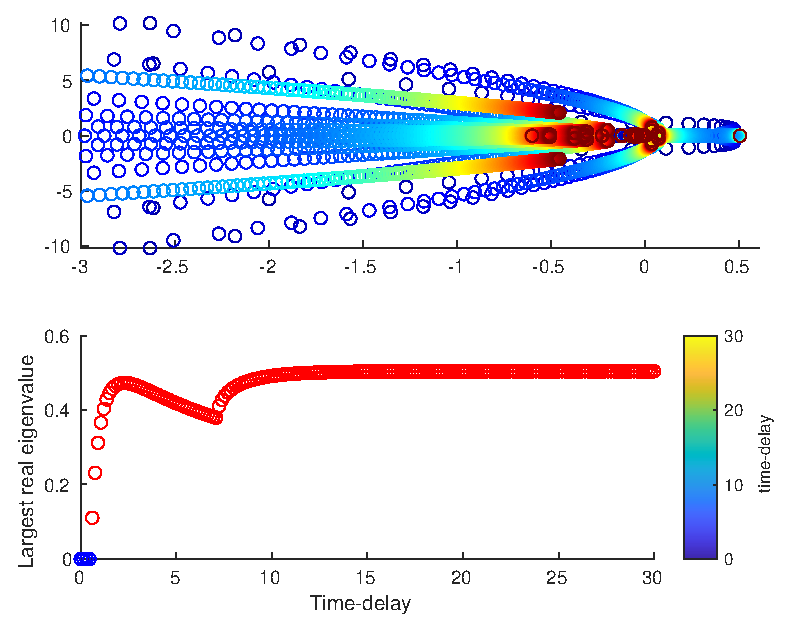
\includegraphics[width=\textwidth]{img/Fig_dump/tau_root_locusLQRDiffIntegralAgnostic_paramsfor_all.eps}
    \label{fig:LQR_root_locus_full_delay}
    \caption{Root locus plot for delays on all plant inputs}
\end{figure}

The controller is quite sensitive to time-delays from the results in figure \ref{fig:LQR_root_locus_full_delay}, becoming unstable if all inputs suffer an input-delay of only 0.3 seconds. If it can be guaranteed that there will be some inputs without delays, some stronger guarantees can be given instead. A delay of 5 seconds can be tolerated if there is no delay in the grate-speed. Sadly, this input that gives a notable improvement is if $v_{grate}$ .


\noindent 
The fact that $v_{grate}$ is one of the most problematic inputs was not something that could be solved in this project. It is especially bad, since it would seem more reasonable that the fans have a lot less variance in their delay compared to the ram and the grates, simply because they are a lot faster. In theory, decreasing the reliance on $v_{grate}$ should make it better, but no solution was found during this project that also resulted in performance that could rival the previous controller. There may be some solution, using a different architecture or bu using a different set of weights. 



\begin{figure}
    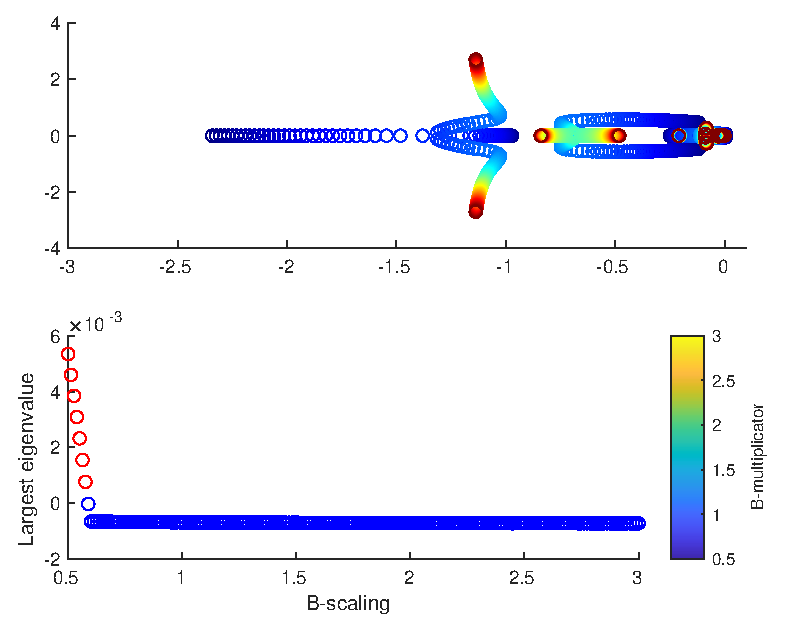
\includegraphics[width=\textwidth]{img/Fig_dump/B_scaling_root_locusLQRDiffIntegralAgnostic_params.eps}
    \label{fig:LQR_root_locus_B}
    \caption{Root locus plot for linear scalings of B}
\end{figure}



\todo[inline]{Check if this is complete @@@}
\begin{figure}
    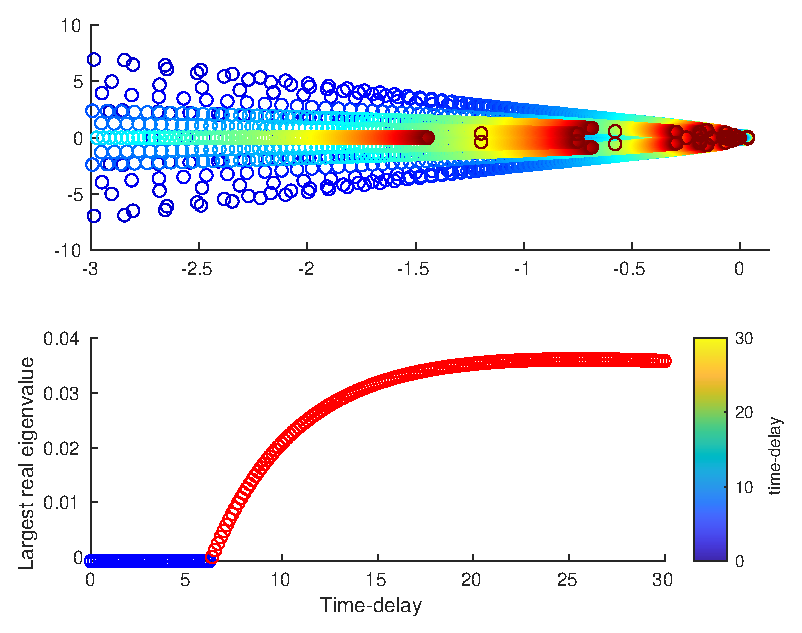
\includegraphics[width=\textwidth]{img/Fig_dump/tau_root_locusLQRDiffIntegralAgnostic_paramsair_diff.eps}
    \label{fig:LQR_root_locus_air_safe}
    \caption{Root locus plot for unmodeled time-delays}
\end{figure}


